\subsection{RMN: Corrimiento químico de $^7$Li}

La medición directa de la estructura atómica local es una tarea compleja. Sin
embargo, algunas técnicas espectroscópicas permiten inferir la estructura local 
debido a la gran dependencia de la propiedad medida con respecto al entorno local, 
como lo es el caso de la RMN. La señal de RMN está caracterizada por un pico 
Voigt, que corresponde a una convolución de una función lorentziana, que 
es intrínseca al fenómeno de RMN, y una función gaussiana, debida al detector
\cite{higinbotham2001}. Cada núcleo en particular introduce un corrimiento a la 
señal, corrimiento químico, que depende del apantallamiento electromagnético 
producido por el entorno local y, por lo tanto, por la estructura local. Luego,
el espectro total obtenido para una muestra es la suma de las contribuciones 
procedentes de todos los átomos de $^7$Li de la estructura. En un trabajo previo,
Key \textit{et al.} \cite{key2009} prepararon estructuras de LiSi a diferentes 
concentraciones de litio y midieron los espectros de corrimiento químico del 
$^7$Li. En estas mediciones, Key \textit{et al.} \cite{key2009} le asignaron un 
pico en 18 ppm al corrimiento químico del átomo de $^7$Li cercano a un Si enlazado. 
Por otro lado, atribuyeron el pico en 6 ppm a un átomos de $^7$Li cercano a un Si 
aislado. Sin embargo, no está claro como interpretar la ocurrencia de picos entre 
6 y 18 ppm, que de hecho se observan en las mediciones de RMN de estructuras 
amorfas de Li-Si.

El modelo de vecinos más cercanos que se propone para emular e interpretar las 
mediciones de espectros de corrimiento químico de $^7$Li en aleaciones de LiSi 
define el corrimiento químico del $i$-ésimo átomo de Li como
\begin{equation}\label{eq:dli}
    \delta_{i} = \frac{1}{N_i^{\text{Si}}} \sum^{N_i^{\text{Si}}}_{\alpha} \delta_{\text{Key}}(\alpha),
\end{equation}
donde
\begin{equation}\label{eq:dkey}
    \delta_{\text{Key}}(\alpha)=\begin{cases}
    18 \text{ppm} & \text{si } \alpha \text{ es un átomo de Si enlazado}\\
    6 \text{ppm} & \text{si } \alpha \text{ es un átomo de Si aislado} 
    \end{cases}
\end{equation}

La ecuación \ref{eq:dkey} es una formulación matemática a la hipótesis planteada
por los experimentalistas \cite{key2009} que asumen que el corrimiento químico 
se produce esencialmente por dos categorías de iones de Li: aquellos que se 
encuentran próximos a átomos de Si que están enlazados a otros átomos de Si (18 
ppm), y aquellos que se encuentran próximos a Si que están aislados (6 ppm).

La sumatoria en la ecuación \ref{eq:dli} considera a los vecinos más cercanos de 
Si al átomo $i$-ésimo ($N_i^{\text{Si}}$) y $\delta_{\text{Key}}$ se define 
considerando los corrimientos propuestos por Key \textit{et al.} \cite{key2009},
como se discutió previamente. Para determinar los vecinos más cercanos de Si 
se considera una distancia de corte que se elige como la posición del mínimo 
entre el primer y el segundo pico de la RDF parcial de Si-Li, que es 
aproximadamente 3.4 \AA. De manera similar, para el enlace de Si se considera una 
distancia de corte de 3.0 \AA, que es la posición del mínimo entre el primer y el 
segundo pico de la RDF parcial de Si-Si.

El espectro total de RMN se construye como un histograma de picos cuyas posiciones
vienen dadas por la ecuación \ref{eq:dli}. Este histograma se construye sumando 
\textit{kernels} Voigt ($V$) centrados en $\delta_i$ sobre todos los átomos de Li
en la estructura,
\begin{equation}\label{eq:nmr}
    I(x) = \sum_{i} V(x, \delta_{i}, \sigma, \gamma),
\end{equation}
donde $x$ es el corrimiento químico, $\sigma$ es la desviación estándar de la 
componente gaussiana debida al detector y $\gamma$ es el ancho medio a la altura 
media de la componente lorentziana que es intrínseca al fenómeno de RMN. Estos 
dos parámetros se ajustan a los datos experimentales. Por último, se promediaron
los resultados sobre las estructuras obtenidas en las trayectorias de dinámica 
molecular.

En la Figura \ref{fig:viz} se muestra una celda unidad simplificada en dos
dimensiones con condiciones periódicas de contorno para explicar el modelo
de vecinos más cercanos de las ecuaciones \ref{eq:dli}, \ref{eq:dkey} y \ref{eq:nmr}
para predecir los resultados del corrimiento químico de RMN para espectros 
del sistema Li-Si.
\begin{figure}[h!]
    \centering
    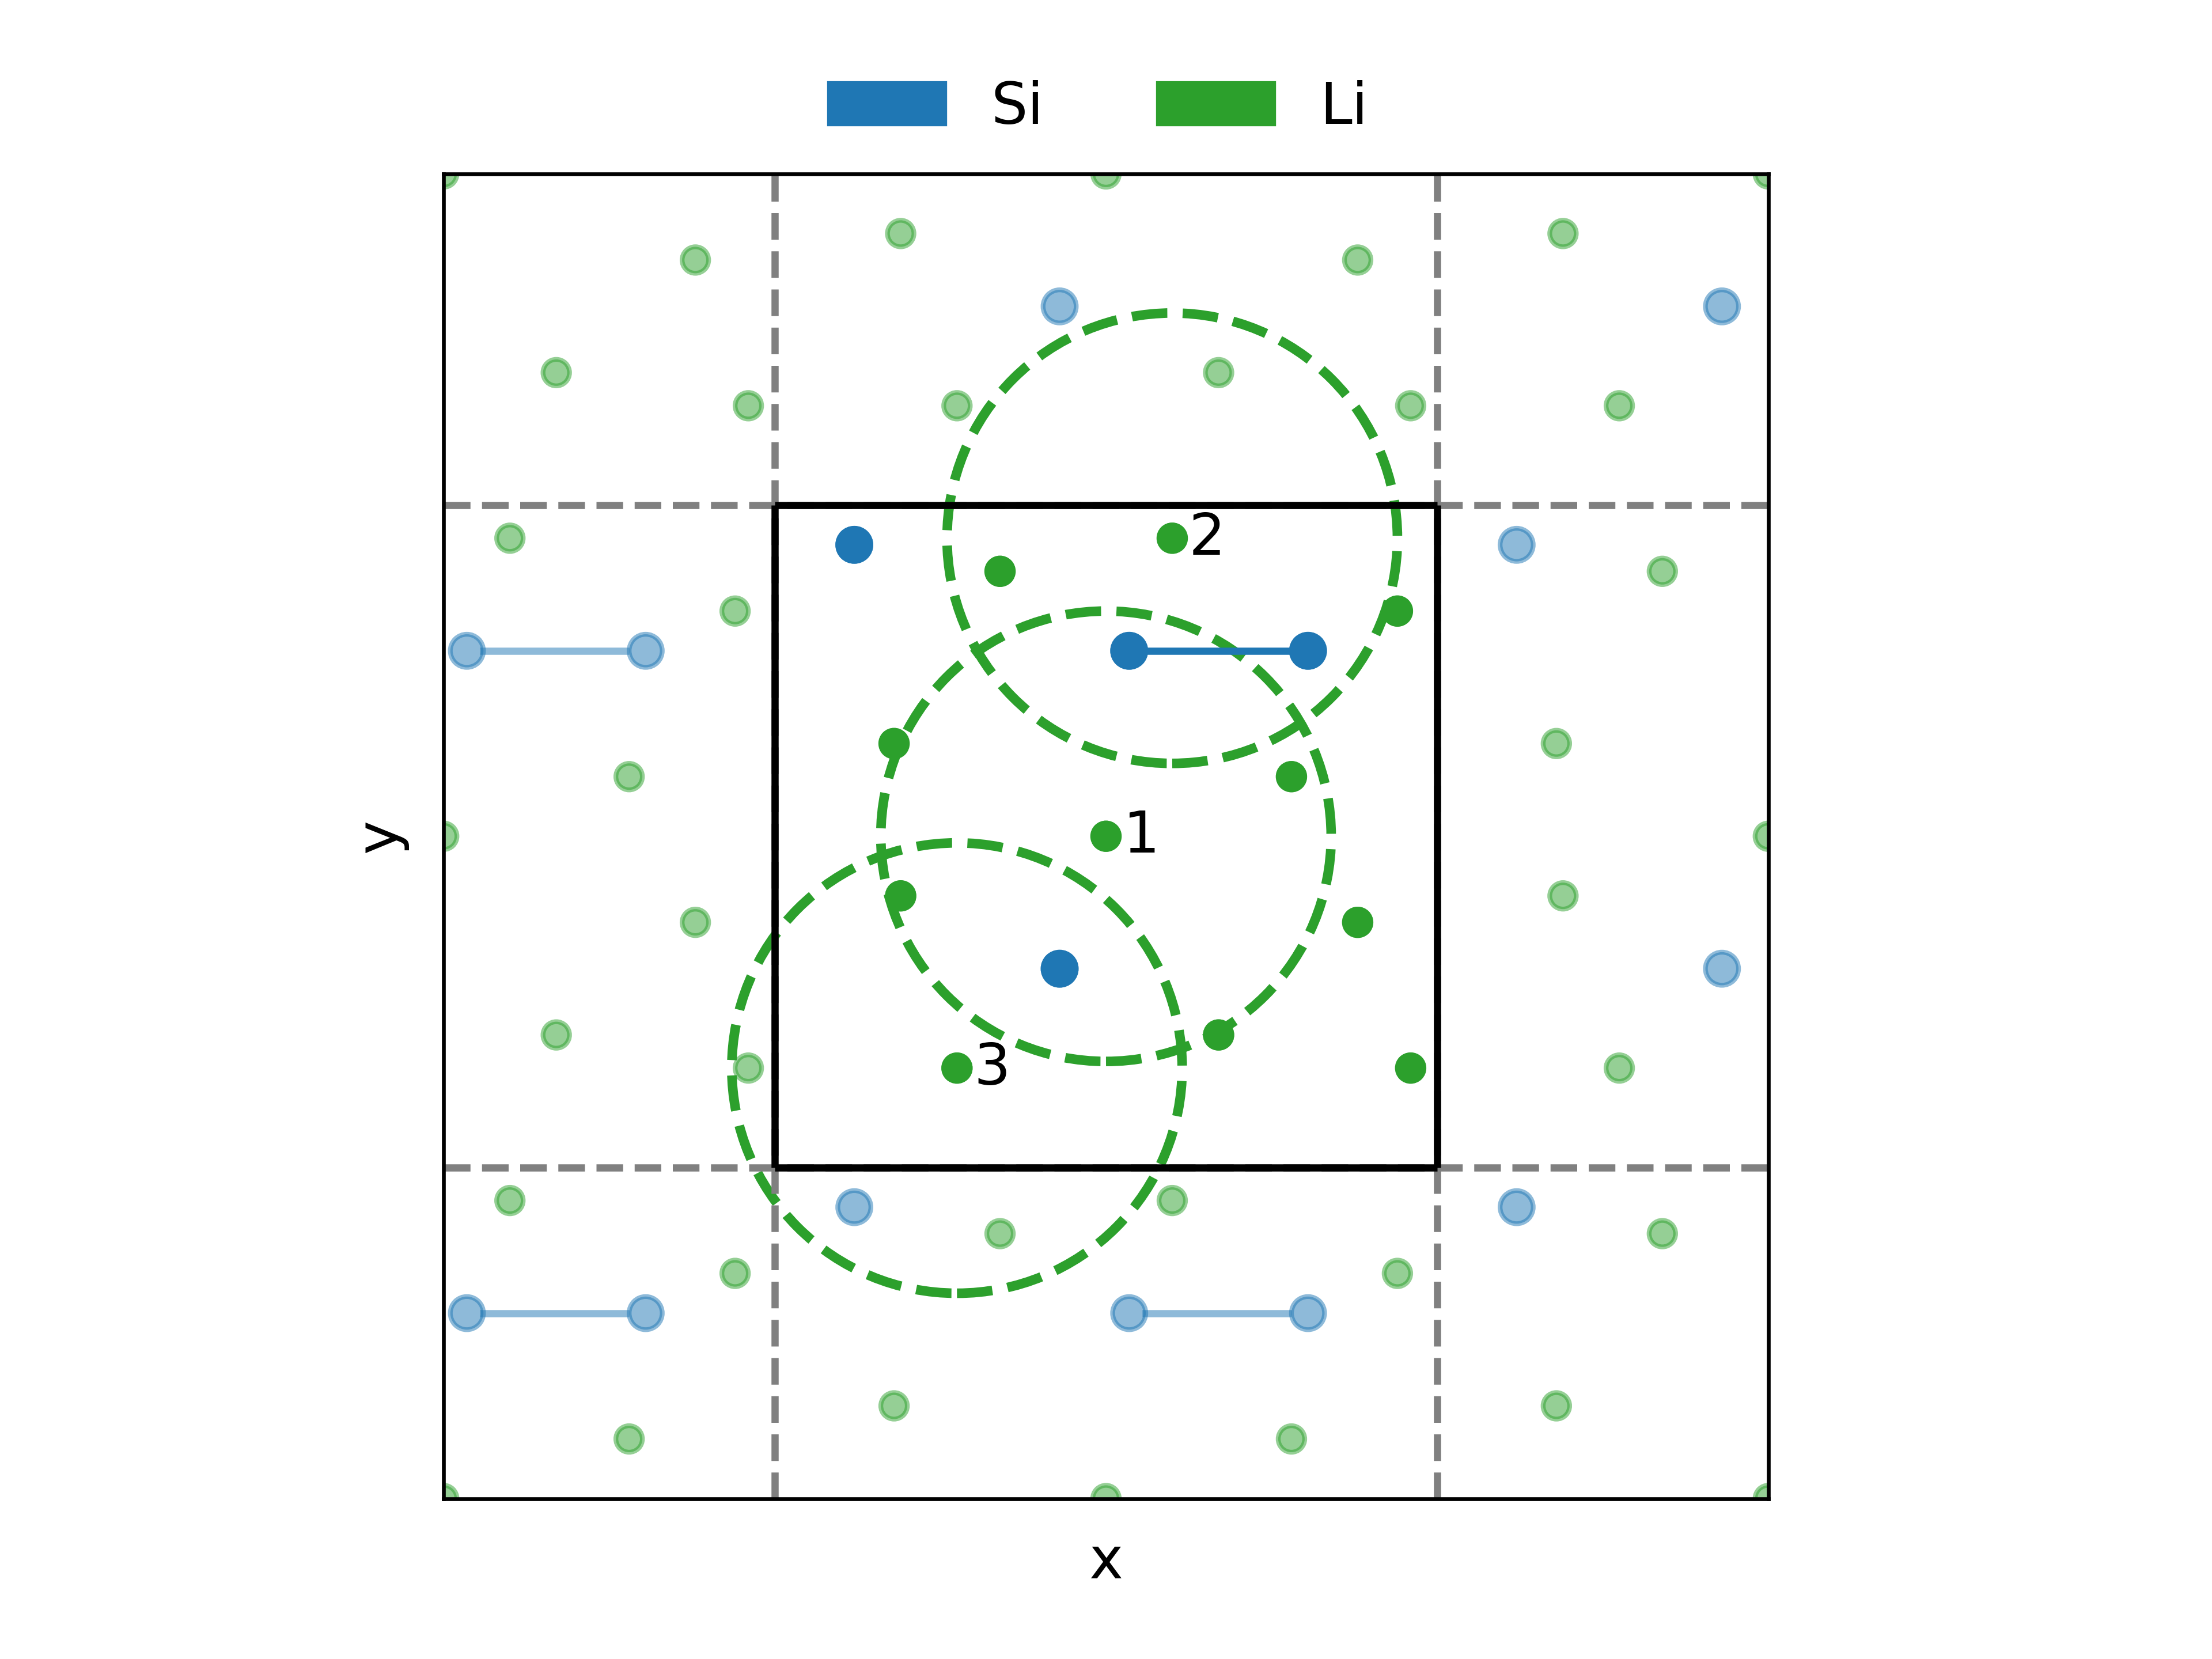
\includegraphics[width=.7\textwidth]{Silicio/prediccion/resultados/nmr/viz.png}
    \caption{Diagrama para explicar el modelo de vecinos más cercanos que predice los
    espectros de RMN en sistemas Li--Si.} 
    \label{fig:viz}
\end{figure}
Cada átomo de Li contribuye con un pico Voigt, donde su centro
depende del tipo de átomos de Si (enlazado o aislado) en su primera esfera de 
coordinación. El radio de corte para dicha esfera es igual a 3.4 \AA\ para todas 
las concentraciones, esto puede verse en la RDF parcial de Si-Si en la Figura 
\ref{fig:prdfs}. Por ejemplo, para el átomo de Li $1$ se tiene
\begin{equation}
    \delta_1 = \frac{18 \text{ppm} + 6 \text{ppm}}{2} = 12 \text{ppm},
\end{equation}
donde 18 ppm y 6 ppm vienen del átomo enlazado y del aislado, respectivamente,
que se observa en su primera esfera de coordinación. De la misma manera, para 
el átomo $2$ de Li se tiene 
\begin{equation}
    \delta_2 = \frac{18 \text{ppm} + 18 \text{ppm}}{2} = 18 \text{ppm},
\end{equation}
y para el átomo $3$ de Li
\begin{equation}
    \delta_3 = \frac{6 \text{ppm} + 6 \text{ppm}}{2} = 6 \text{ppm}.
\end{equation}
Luego, la intensidad del espectro generada por estos tres átomos es la suma
de sus contribuciones con picos Voigt centrados en los corrimientos químicos
calculados
\begin{equation}
    I = V_1(12\text{ppm}) + V_2(18\text{ppm}) + V_3(6\text{ppm}) + ...,
\end{equation}
y así puede considerarse el resto de los átomos de Li en la estructura.

Como primera prueba a este modelo se presenta el corrimiento químico de $^7$Li 
predicho para las estructuras cristalinas en la Figure \ref{fig:c-nmr}. 
\begin{figure}[h!]
    \centering
    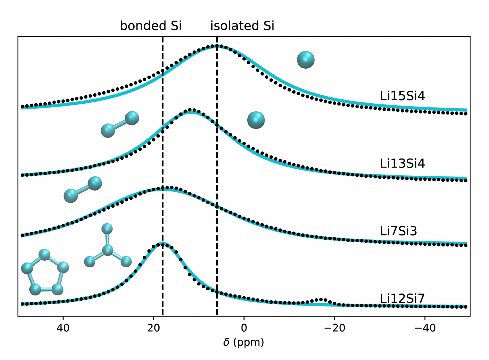
\includegraphics[width=.7\textwidth]{Silicio/prediccion/resultados/nmr/c-nmr.png}
    \caption{Espectros de corrimiento químico de $^7$Li para aleaciones 
    cristalinas. Los puntos corresponden a las mediciones de Key \textit{et al.}
    y las líneas al modelo de vecinos más cercanos. Las líneas verticales indican las 
    contribuciones del Si enlazado y aislado. Las barras de error son menores que
    el ancho de las líneas.}
    \label{fig:c-nmr}
\end{figure}
Las estructuras cristalinas se extrajeron del Materials Project 
\cite{materials_project} y el ancho de los picos se ajustó a la precisión de los 
experimentos de Key \textit{et al.} \cite{key2009} una vez que se determinó el 
centro de los mismos con el modelo de las ecuaciones \ref{eq:dli} y \ref{eq:dkey}.
Las predicciones del modelo se muestran con curvas continuas mientras que las 
mediciones de Key se corresponden con los puntos. Para todas las aleaciones se 
reproduce el centro del pico con gran precisión. En las aleaciones 
Li$_{12}$Si$_7$ y Li$_7$Si$_3$ todos los átomos de Si se encuentran enlazados. 
En la primera de ellas forman pentágonos de cinco átomos de estrellas de cuatro, 
mientras que en la segunda todos los enlaces son mancuernas. Esto hace que las 
contribuciones de todos los átomos de Li se centren en 18 ppm en el modelo. Para 
la aleación Li$_{15}$Si$_4$ sólo se tienen Si aislados, lo cual centra todas las
contribuciones en 6 ppm. Mientras tanto, hay una coexistencia de Si enlazados y 
Si aislados en Li$_{13}$Si$_4$ que produce contribuciones intermedias al espectro,
consistente con el experimento.

Habiéndose obtenido estos resultados prometedores para las estructuras cristalinas,
se centra la discusión que sigue en estructuras amorfas, que son las que 
usualmente se encuentran en los experimentos electroquímicos. En este caso se 
calculan los espectros de corrimiento químico de $^7$Li con el modelo de vecinos 
más cercanos utilizando las estructuras amorfas de Li$_x$Si simuladas con 
dinámica molecular. Se consideran valores de $x$ que pueden relacionarse con los 
potenciales a los cuales Key \textit{et al.} realizaron las mediciones 
\cite{key2009}. Para facilitar la comparación de las predicciones del modelo con 
los datos experimentales, se incluyó un pico a -0.3 ppm que representa la 
interfase electrolito sólido (SEI), como sugieren los autores citados. Estos 
resultados se los muestra en la Figura \ref{fig:a-nmr} que, a pesar de algunas 
diferencias que se explican a continuación, presenta una concordancia razonable
entre los resultados computacionales y experimentales.
\begin{figure}[h!]
    \centering
    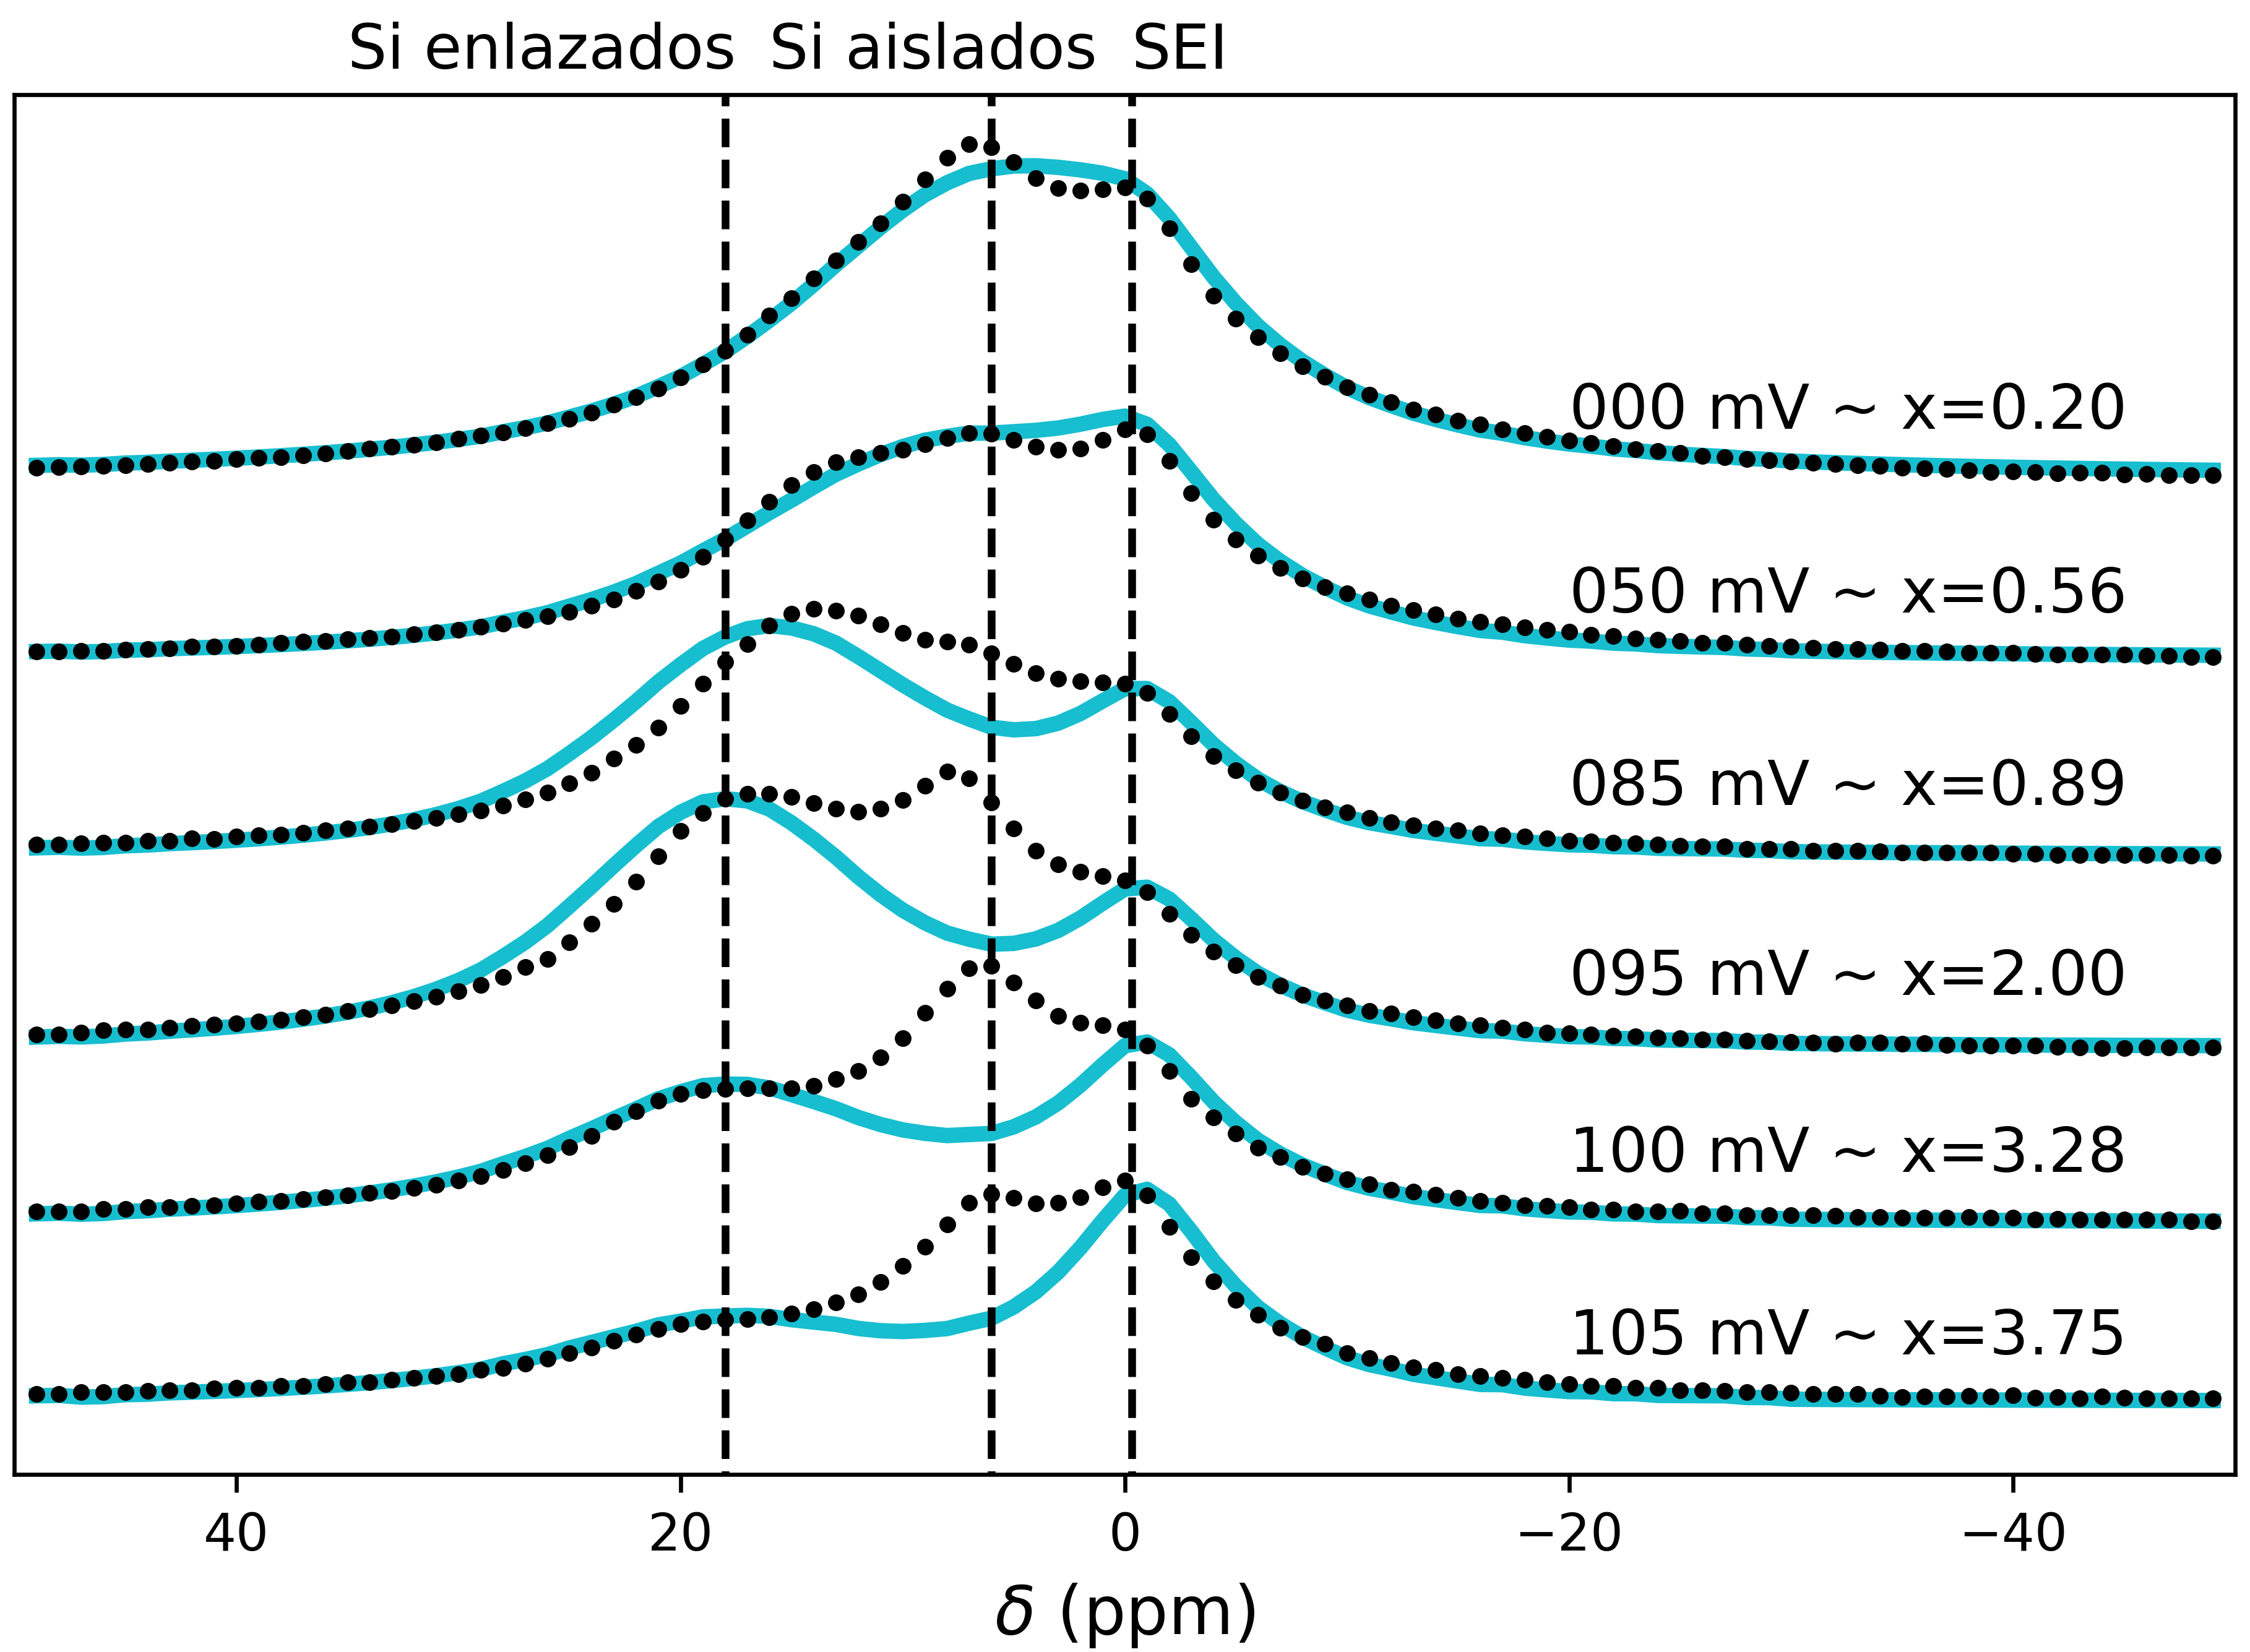
\includegraphics[width=.7\textwidth]{Silicio/prediccion/resultados/nmr/a-nmr.png}
    \caption{Espectros de corrimiento químico de $^7$Li para estructuras amorfas.
    Los puntos corresponden a las mediciones de Key \textit{et al.}. Los 
    resultados del modelo se representan con líneas continuas y se añade una 
    contribución de la SEI para comparar con el experimento. Las líneas verticales 
    indican las contribuciones de la SEI y de los átomos de Si enlazados o 
    aislados. Las barras de error son menores que el ancho de las líneas. Las 
    discrepancias a 6 ppm pueden deberse a una litiación inhomogénea en los 
    experimentos, como se explica en la referencia \cite{key2009}.} 
    \label{fig:a-nmr}
\end{figure}
Esto es particularmente cierto para el caso del pico en 18 ppm, donde el modelo 
es capaz de imitar su desplazamiento a 6 ppm a concentraciones altas. Este cambio
es la evidencia más clara que sustenta la visión atomística actual del sistema: 
Al principio de la litiación las estructuras están conformadas por átomos de Si 
enlazados, luego, a concentraciones intermedias, hay una coexistencia entre Si 
enlazados y Si aislados y, a concentraciones altas de litio, hay una predominancia
de estos últimos sobre los primeros.

Hay una mejor concordancia entre las predicciones del modelo y los experimentos
a concentraciones altas de Li. A concentraciones bajas de Li, las predicciones del 
modelo muestran una discrepancia considerable con los resultados experimentales.
Sin embargo, esto no debe ser atribuido a una deficiencia del modelo, sino más 
bien a que la litiación en el experimento es sumamente inhomogénea \cite{key2009}.
Esto es, la contribución extra en el espectro experimental a 6 ppm se la atribuye 
a Si aislados en regiones altamente litiadas que no son incluidas en las 
estructuras simuladas. Las simulaciones de dinámica molecular realizadas se 
corresponden a estructuras en equilibrio termodinámico y no tienen en cuenta estas 
fases meta-estables altamente litiadas que aparecen en los experimentos de Key 
\textit{et al.} \cite{key2009} a concentraciones globales de Li bajas.
